\documentclass[11pt]{article}
\usepackage[utf8]{inputenc}	% Para caracteres en español
\usepackage{amsmath,amsthm,amsfonts,amssymb,amscd}
\usepackage{multirow,booktabs}
\usepackage[table]{xcolor}
\usepackage{fullpage}
\usepackage{lastpage}
\usepackage{enumitem}
\usepackage{fancyhdr}
\usepackage{mathrsfs}
\usepackage{wrapfig}
\usepackage{setspace}
\usepackage{calc}
\usepackage{multicol}
\usepackage{cancel}
\usepackage[retainorgcmds]{IEEEtrantools}
\usepackage[margin=1cm]{geometry}
\usepackage{amsmath}
\newlength{\tabcont}
\setlength{\parindent}{0.0in}
\setlength{\parskip}{0.05in}
\usepackage{empheq}
\usepackage{framed}
\usepackage[most]{tcolorbox}
\usepackage{xcolor}
\usepackage{graphicx}
\usepackage{listings}
% -- Basic formatting
\usepackage[utf8]{inputenc}
\usepackage[english]{babel}
\usepackage{times}
\usepackage{caption}
\usepackage{subcaption}
\usepackage{placeins}
\setlength{\parindent}{0pt}
\usepackage{indentfirst}% -- Defining colors:
\usepackage[dvipsnames]{xcolor}
\definecolor{codegreen}{rgb}{0,0.6,0}
\definecolor{codegray}{rgb}{0.5,0.5,0.5}
\definecolor{codepurple}{rgb}{0.58,0,0.82}
\definecolor{backcolour}{rgb}{0.95,0.95,0.92}% Definig a custom style:
\lstdefinestyle{mystyle}{
    backgroundcolor=\color{backcolour},   
    commentstyle=\color{codepurple},
    keywordstyle=\color{NavyBlue},
    numberstyle=\tiny\color{codegray},
    stringstyle=\color{codepurple},
    basicstyle=\ttfamily\footnotesize\bfseries,
    breakatwhitespace=false,         
    breaklines=true,                 
    captionpos=t,                    
    keepspaces=true,                 
    numbers=left,                    
    numbersep=5pt,                  
    showspaces=false,                
    showstringspaces=false,
    showtabs=false,                  
    tabsize=2
}% -- Setting up the custom style:
\lstset{style=mystyle}
\lstset{
  style=mystyle,
  framexleftmargin=3.5mm,
  rulesepcolor=\color{black},
  linewidth=0.6\linewidth,
  xleftmargin=12pt,
  aboveskip=12pt,
  belowskip=12pt
}
\colorlet{shadecolor}{orange!15}
\parindent 0in
\parskip 1pt
\geometry{margin=1in, headsep=0.25in}
\theoremstyle{definition}
\newtheorem{defn}{Definition}
\newtheorem{reg}{Rule}
\newtheorem{exer}{Exercise}
\newtheorem{note}{Note}
\graphicspath{ {./images/} }
\begin{document}
\setcounter{section}{0}
\title{MIE223 Lecture Notes}

\thispagestyle{empty}

\begin{center}
{\LARGE \bf Advanced Data Science and Fallacies}\\
{\large MIE223}\\
Winter 2025
\end{center}

\section{Potential Data Interpretation Fallacies}
\subsection{Anscombe Quartet: Visualize}
When we look at mean of x, sample variance of x, mean of y, sample variance of y,
correlation between x and y, and linear regression line, the accuracy differs.

If datasets have varying levels of accuracy, the mean, variance, and correlation will be the same. However, the linear regression line will differ.

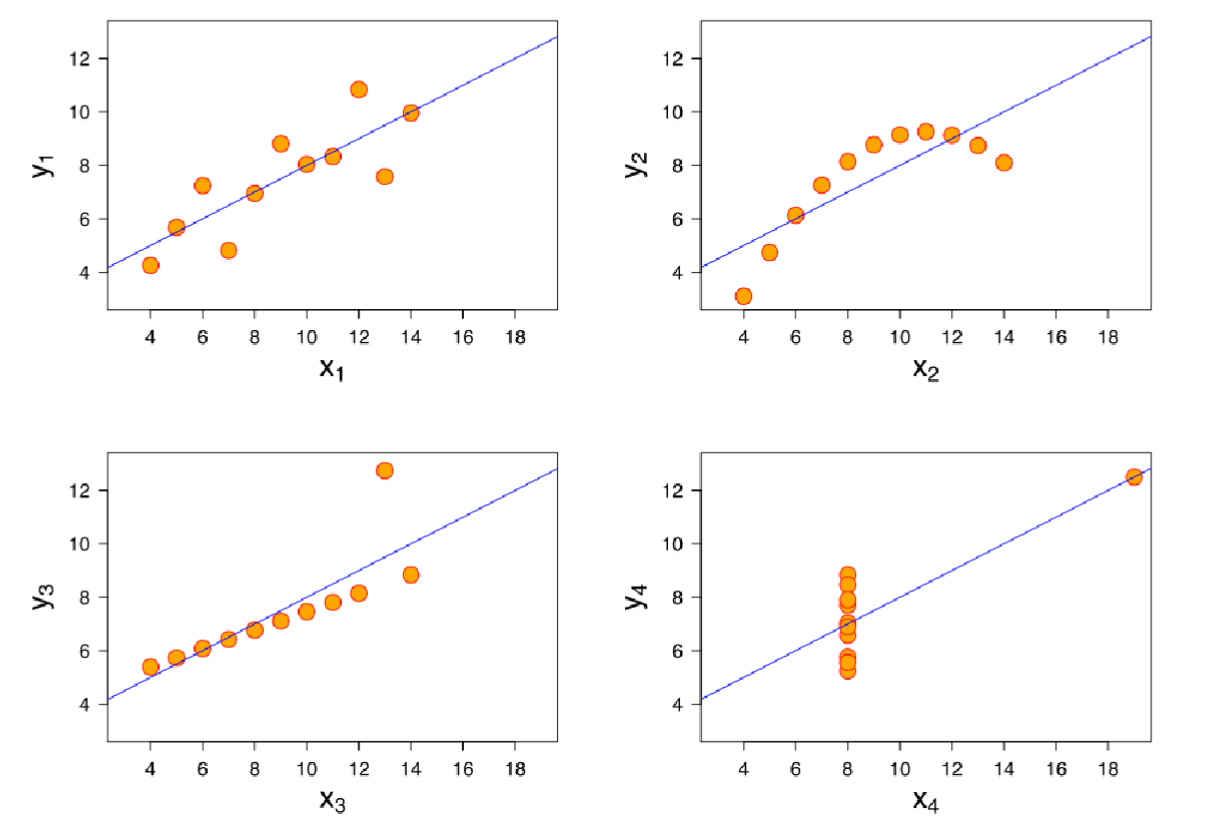
\includegraphics[width=\textwidth]{27.png}

\subsection{Spurious Correlation}

Ratios induce spurious correlations. Solution: compositional data analysis.

x, y, and z are all statistically independent. 
The ratios induce high correlation between them.

Normalizing by a common number (such as in ratios) results in spurious correlation.

\subsection{Confounding Variables}
\begin{itemize}
    \item Beware of (latent) confounding variables
    \begin{itemize}
        \item Averaging over them can hide important trends
    \end{itemize}
\end{itemize}

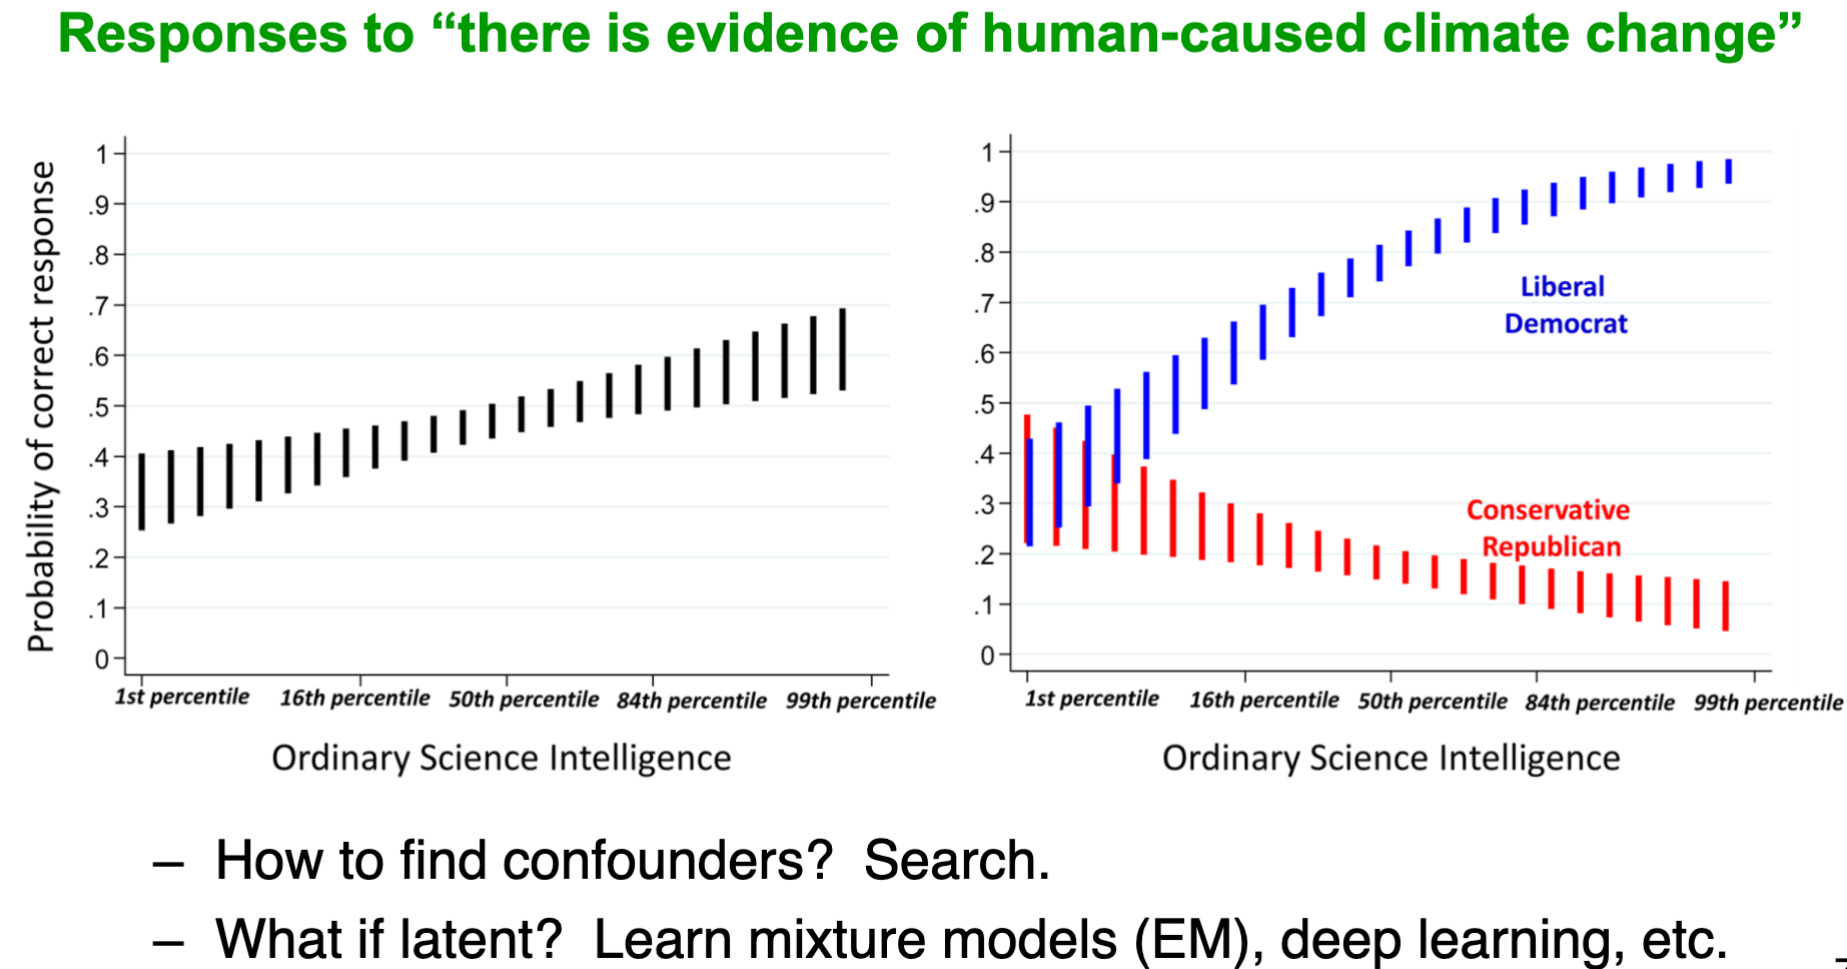
\includegraphics[width=\textwidth]{28.png}

Political affiliation is a confounder. 
Belief in a scientific statement is conditioned on political affiliation.

\subsection{Correctly Normalizing}
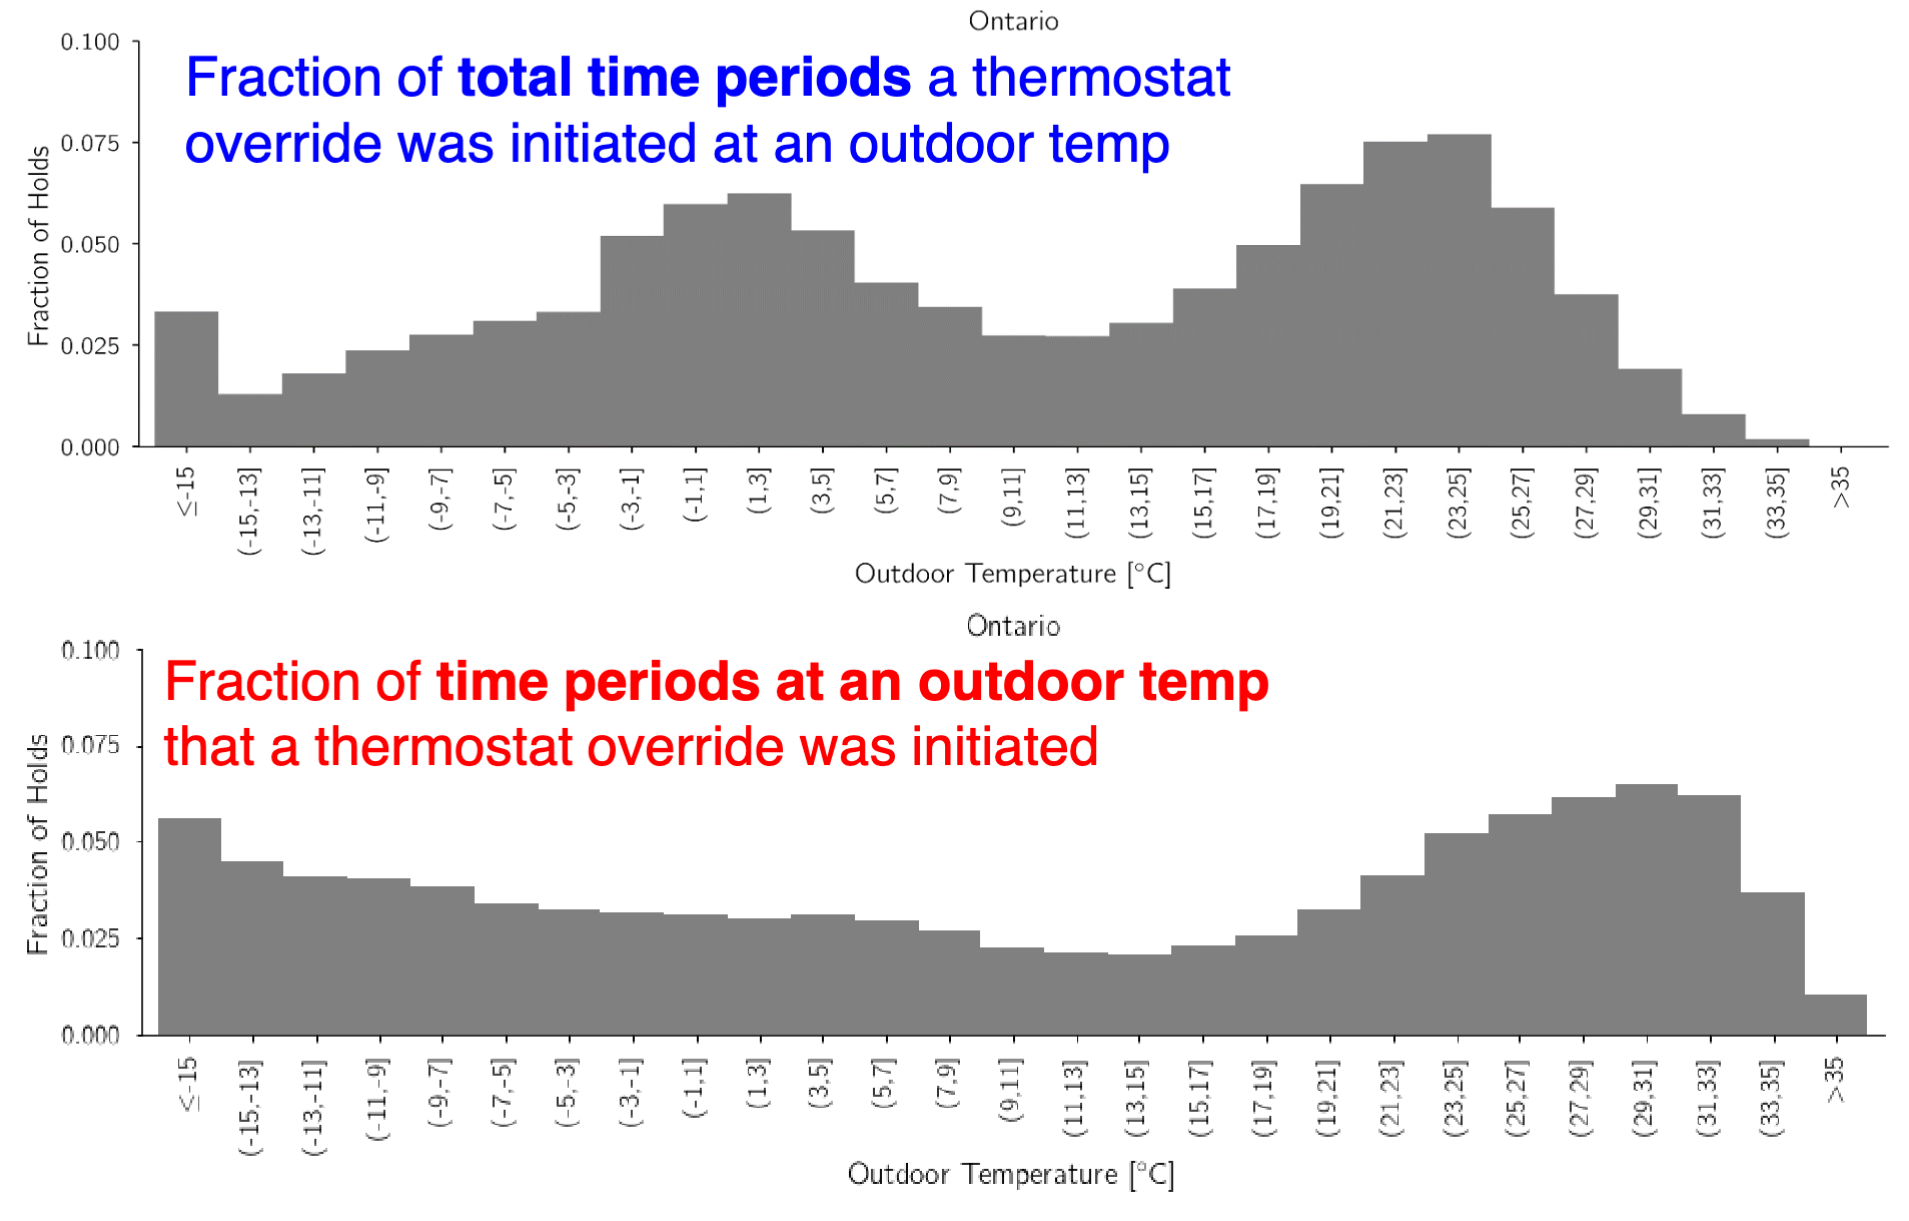
\includegraphics[width=\textwidth]{29.png}

blue 
\begin{itemize}
    \item peaks between 0 and 1 and 23 and 25
    \item Not at certain temperatures with equivalent probability
    \item Looking at a joint measurement not a conditional measurement
\end{itemize}

red 
\begin{itemize}
    \item Normalized by the number of days in each temperature range
\end{itemize}

Fallacies
\begin{itemize}
    \item Don't look at a visualization before you make a hypothesis
\end{itemize}

\subsection{Myth of the Average}
\begin{itemize}
    \item High rate of plane crashes in the 40s
    \begin{itemize}
        \item Seats built for “average” pilot were non-adjustable!
    \end{itemize}
    \item Productivity of publications:
    \item We've averaged out the interesting behaviour of the data
\end{itemize}

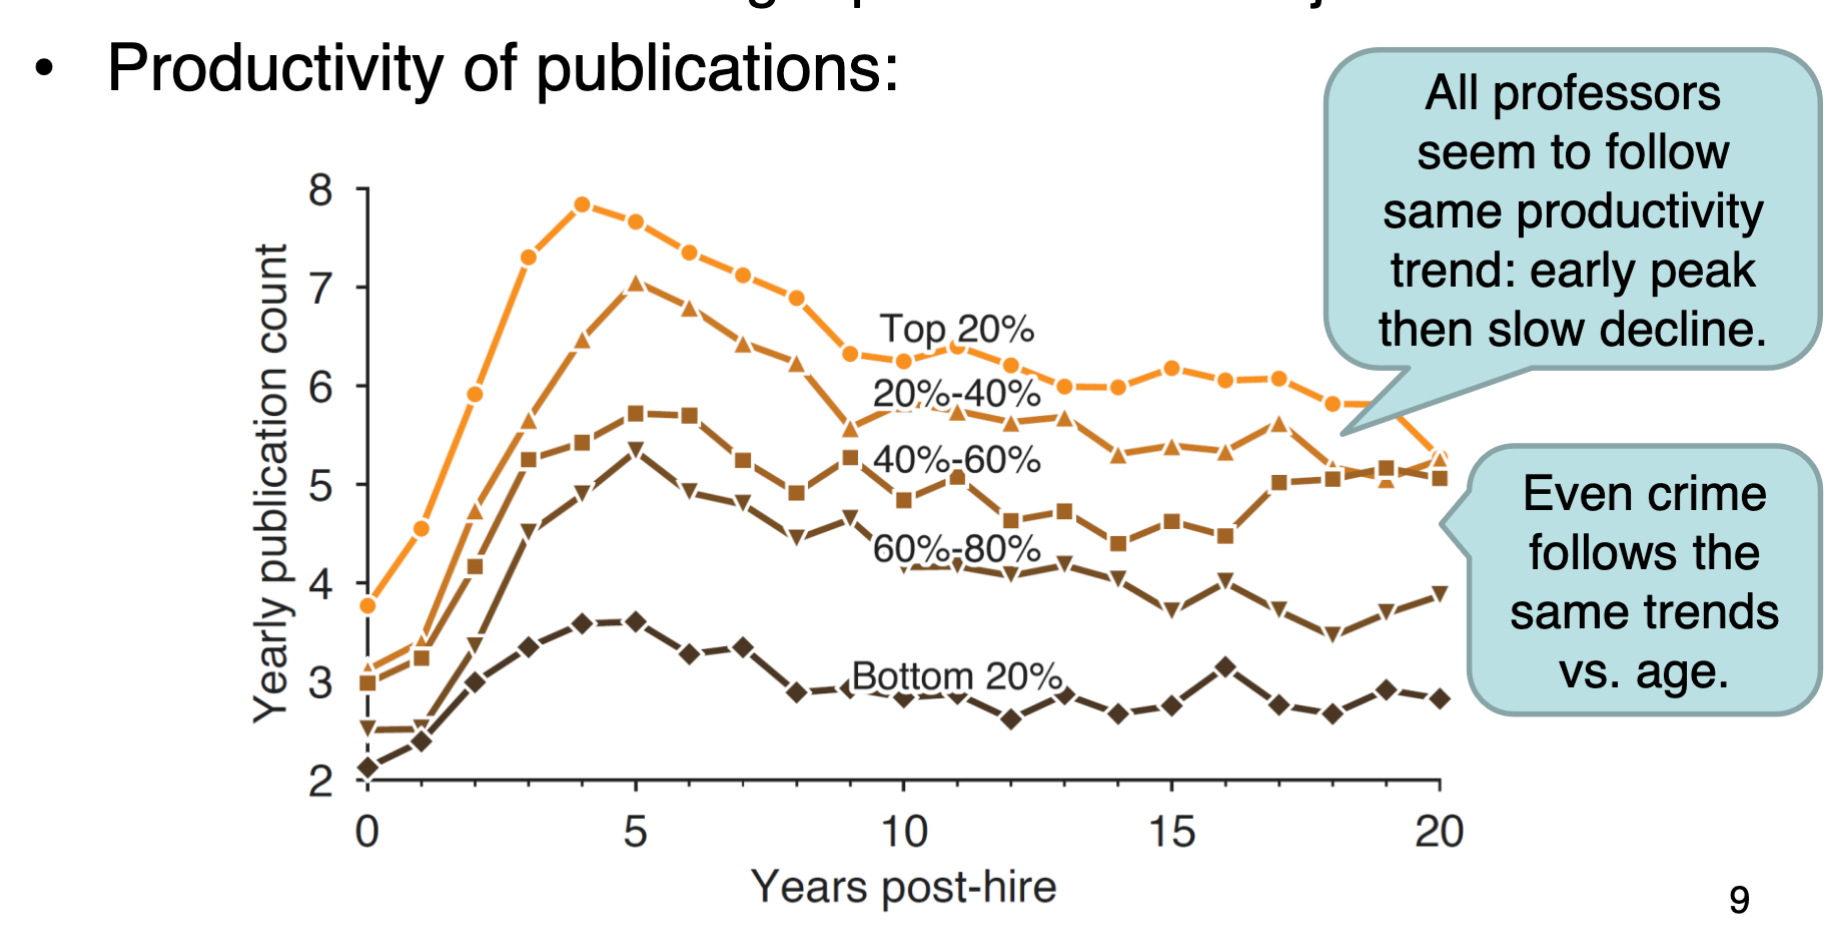
\includegraphics[width=\textwidth]{30.png}

If plot early and later career productivity, a more
complex picture of productivity types emerges...

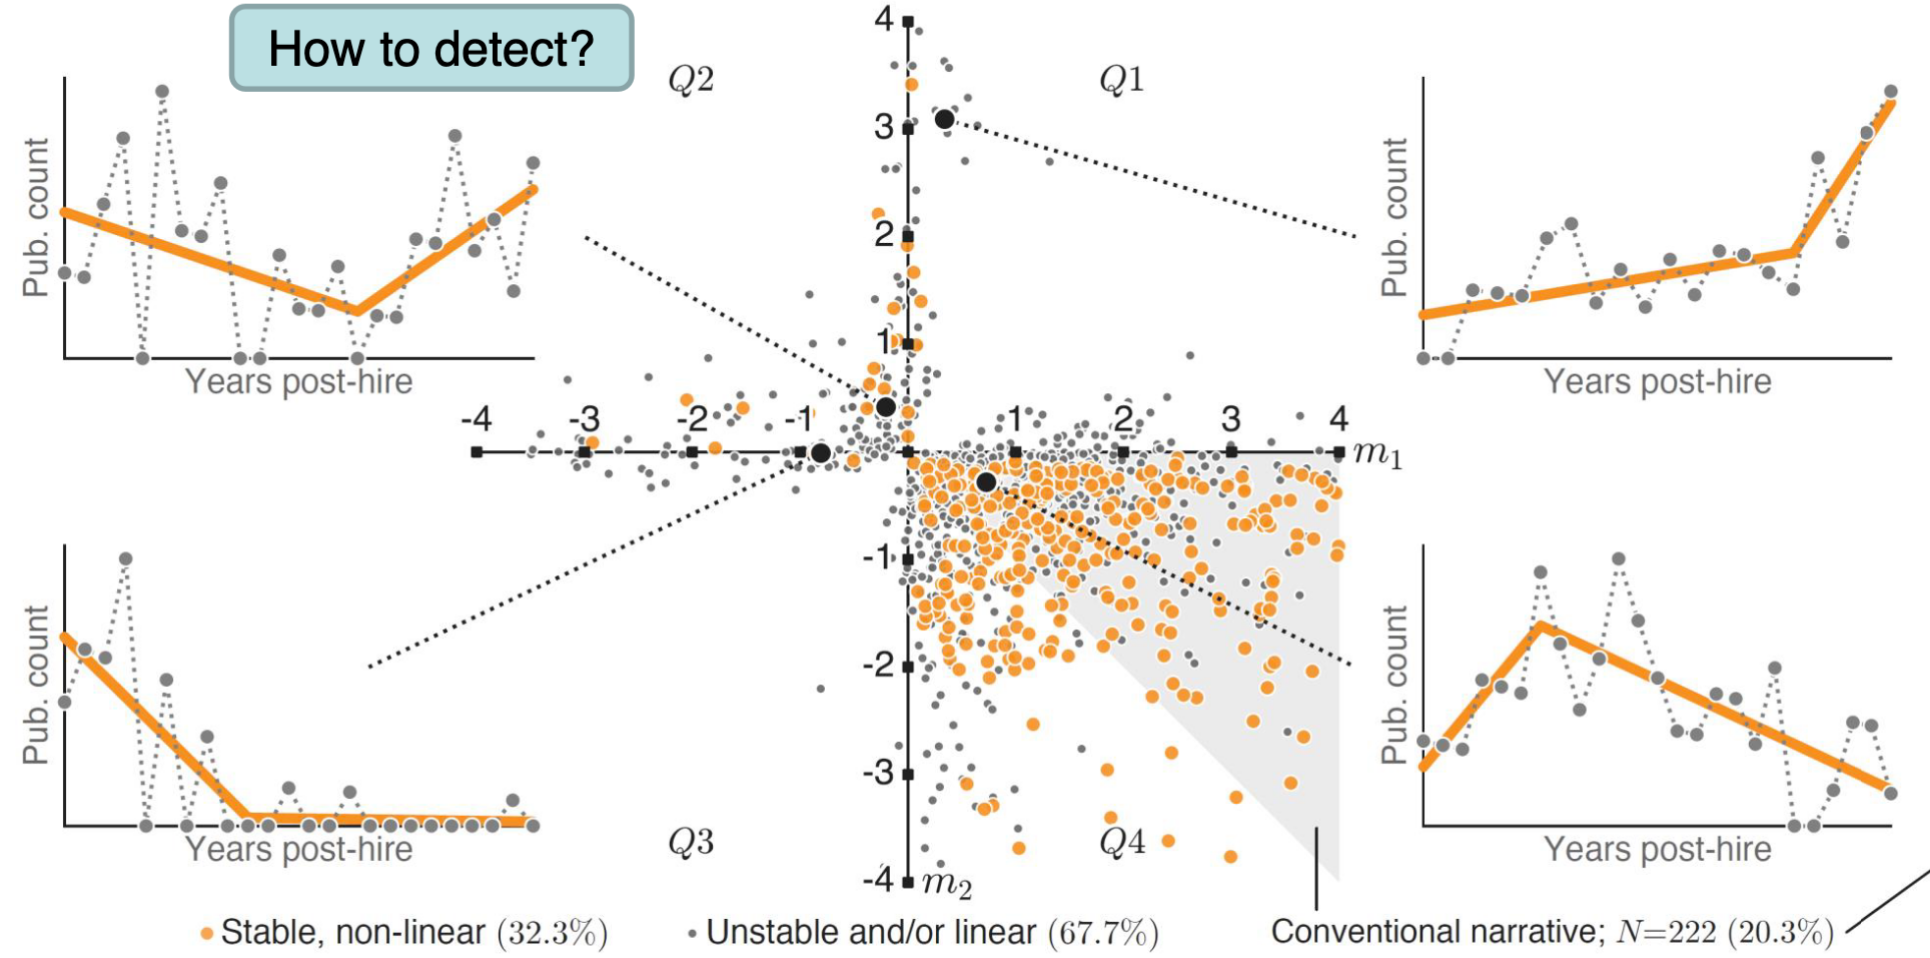
\includegraphics[width=\textwidth]{31.png}

x axis m1, y axis m2.
m1 is positive, m2 is negative.

We didn't see this many different behaviours because of averaging the data.

There are smaller subsets of trends that get shadowed by the majority trend

\subsection{Simpson's Paradox}
Possibly the most problematic issues in data analysis –
unobserved variables and/or sample bias can completely
change your interpretation and decision!

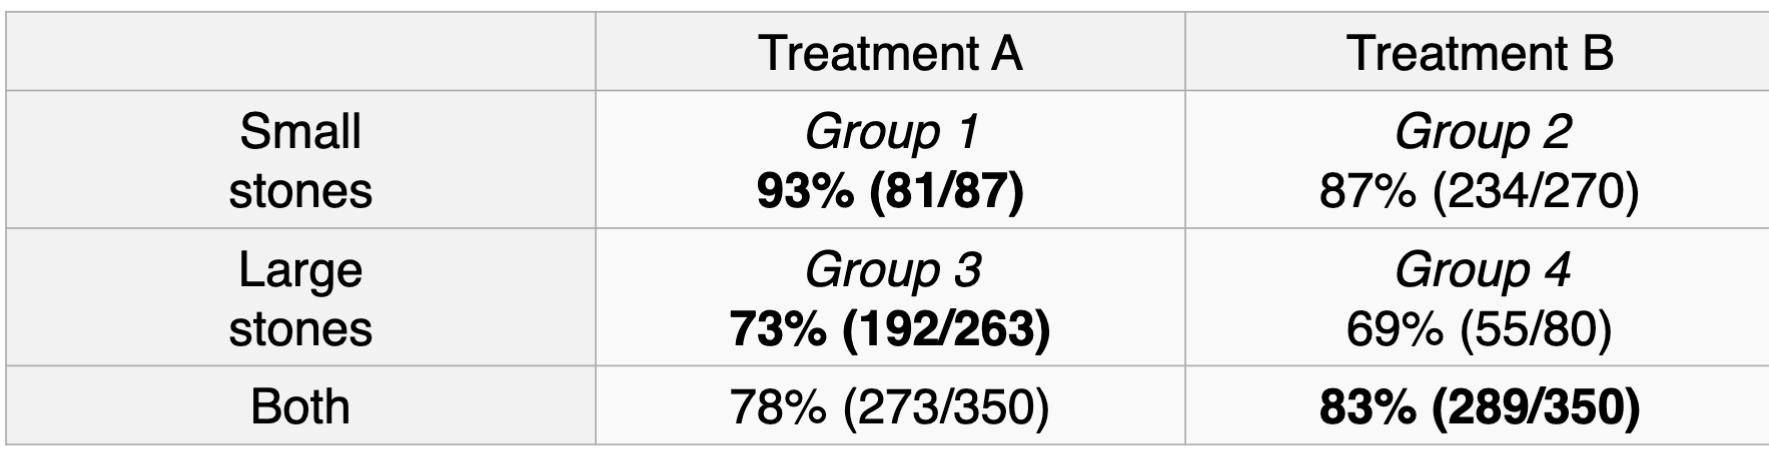
\includegraphics[width=\textwidth]{32.png}

How do resolve this?
– Which answer is correct depends on more knowledge

Aggregating the data can lead to a different conclusion than looking at the data in its entirety.
There is causal interference in the data. Certain doctors
may prescribe differently. Treatment A is more effective but more 
doctors prescribed treatment B to small stones. Small stones 
generally have a higher recovery rate compared to large stones in general.

Look at Wikipedia page on Simpson's paradox that has examples that can be on final exam.

\subsection{Plotting “Right Censored” Time Series Data}

when trying to measure an effect, 
we need to be aware of the horizon effect with time.
if you don't measure long enough you may not see that effect.

\begin{itemize}
    \item Be aware of horizon effects with time
    \begin{itemize}
        \item “right censored”: event may not have happened in all samples
        \begin{itemize}
            \item Or data may be incomplete (people left study, lost track, etc.)
        \end{itemize}
        \item Especially prominent in “survival/failure analysis”
        \begin{itemize}
            \item How long an engine lasts, how long a patient survives, etc.
        \end{itemize}
        \item For plotting: need to make incompleteness in data clear...
    \end{itemize}
\end{itemize}

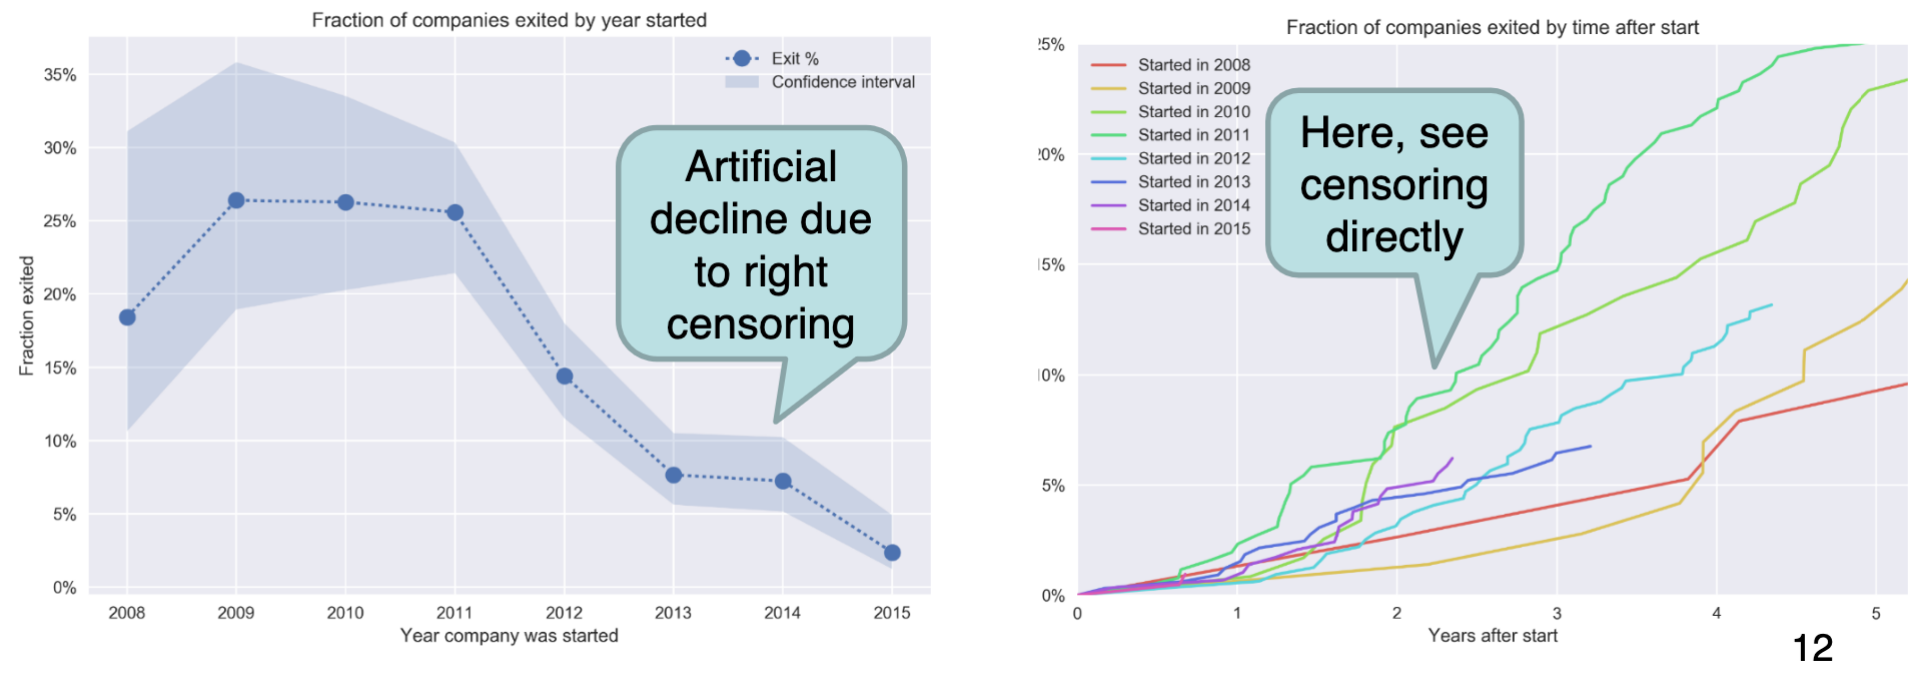
\includegraphics[width=\textwidth]{33.png}

companies that started later have fewer years to exit compared to older startups.

\section{Challenger Disaster}

\subsection{Tufte’s Challenger Example}
Should the Space Shuttle Challenger have been
launched when the launch temperature was -1C?
\begin{itemize}
    \item Hashes show
    post-launch
    damage
    evaluation.
    \item This chart
    does not help
    us answer
    the question.
    Why not?
\end{itemize}

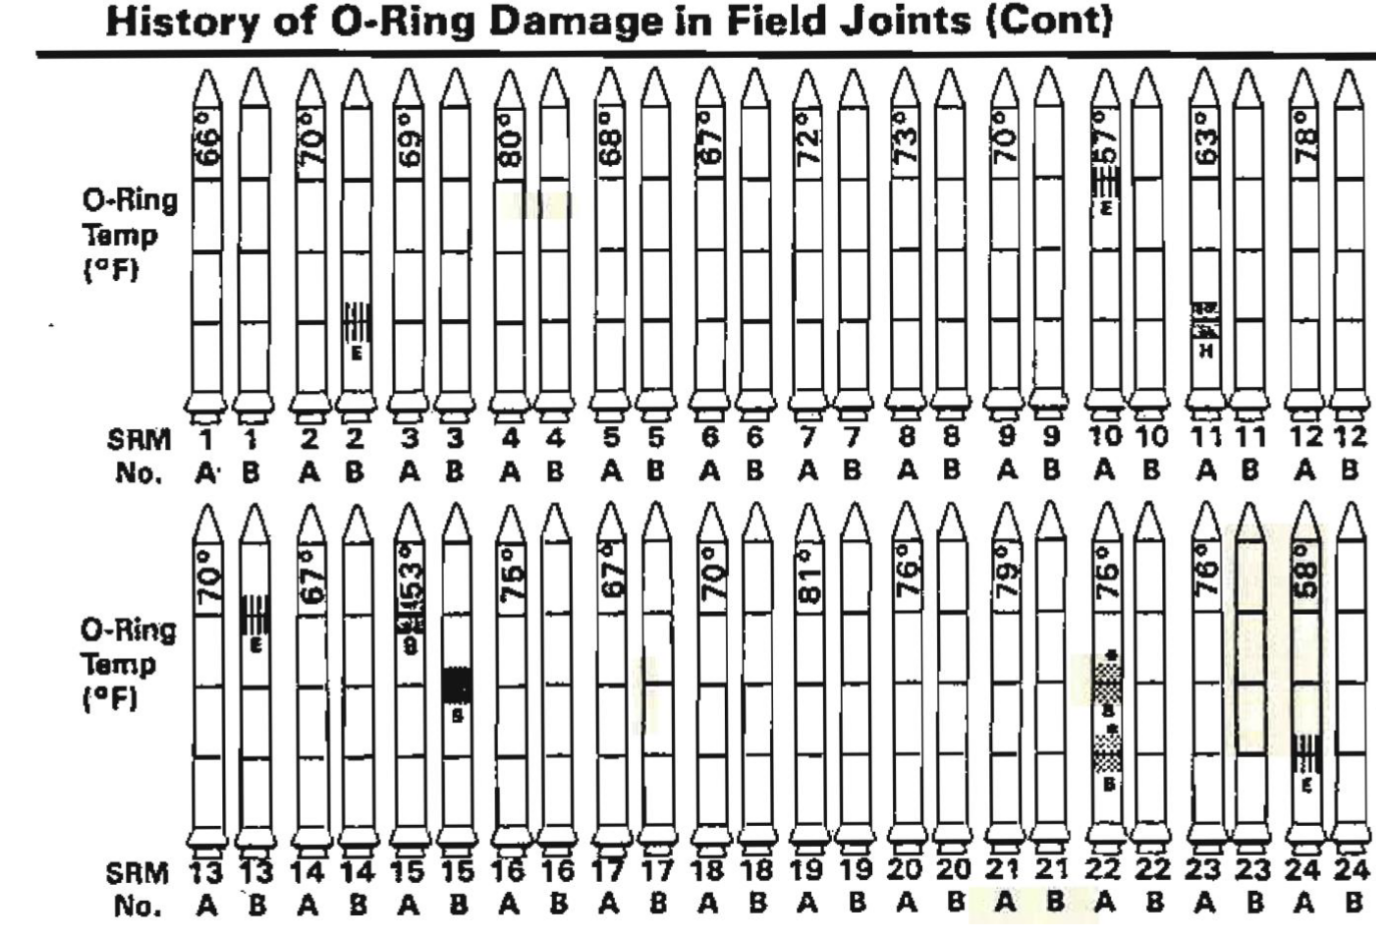
\includegraphics[width=\textwidth]{34.png}

If temperature is what concerns us, let’s reorder by
temperature:

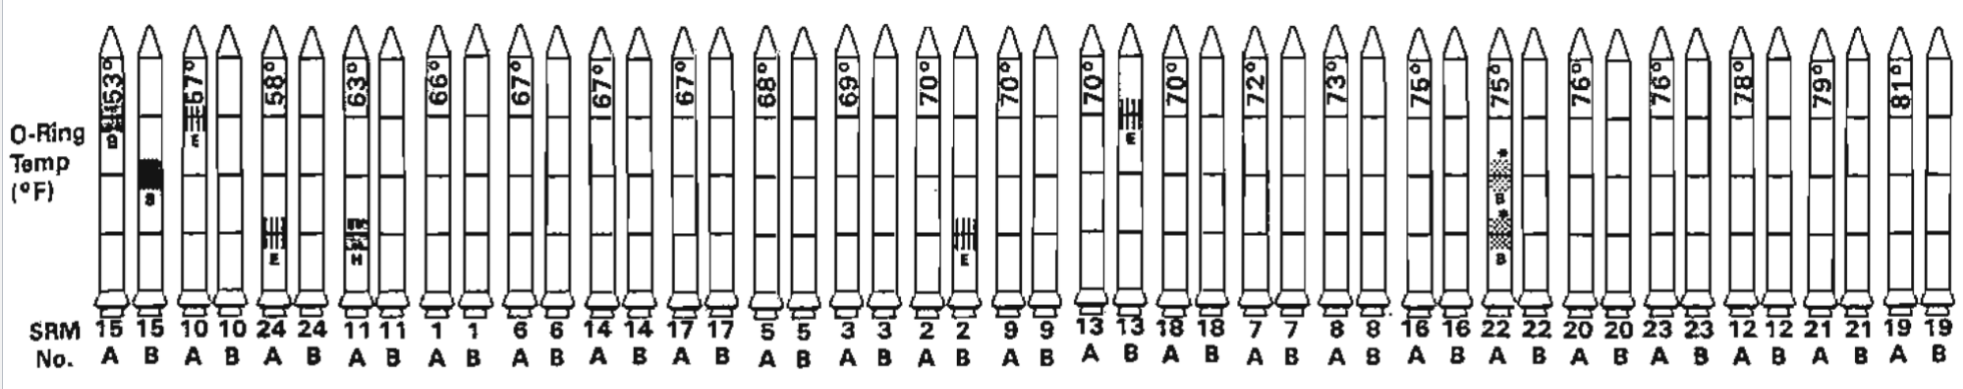
\includegraphics[width=\textwidth]{35.png}

OK, some
concentrated
damage at lower
temperatures, but not
highly conclusive.

Let us accurately represent the temperature scale and
try one more time:

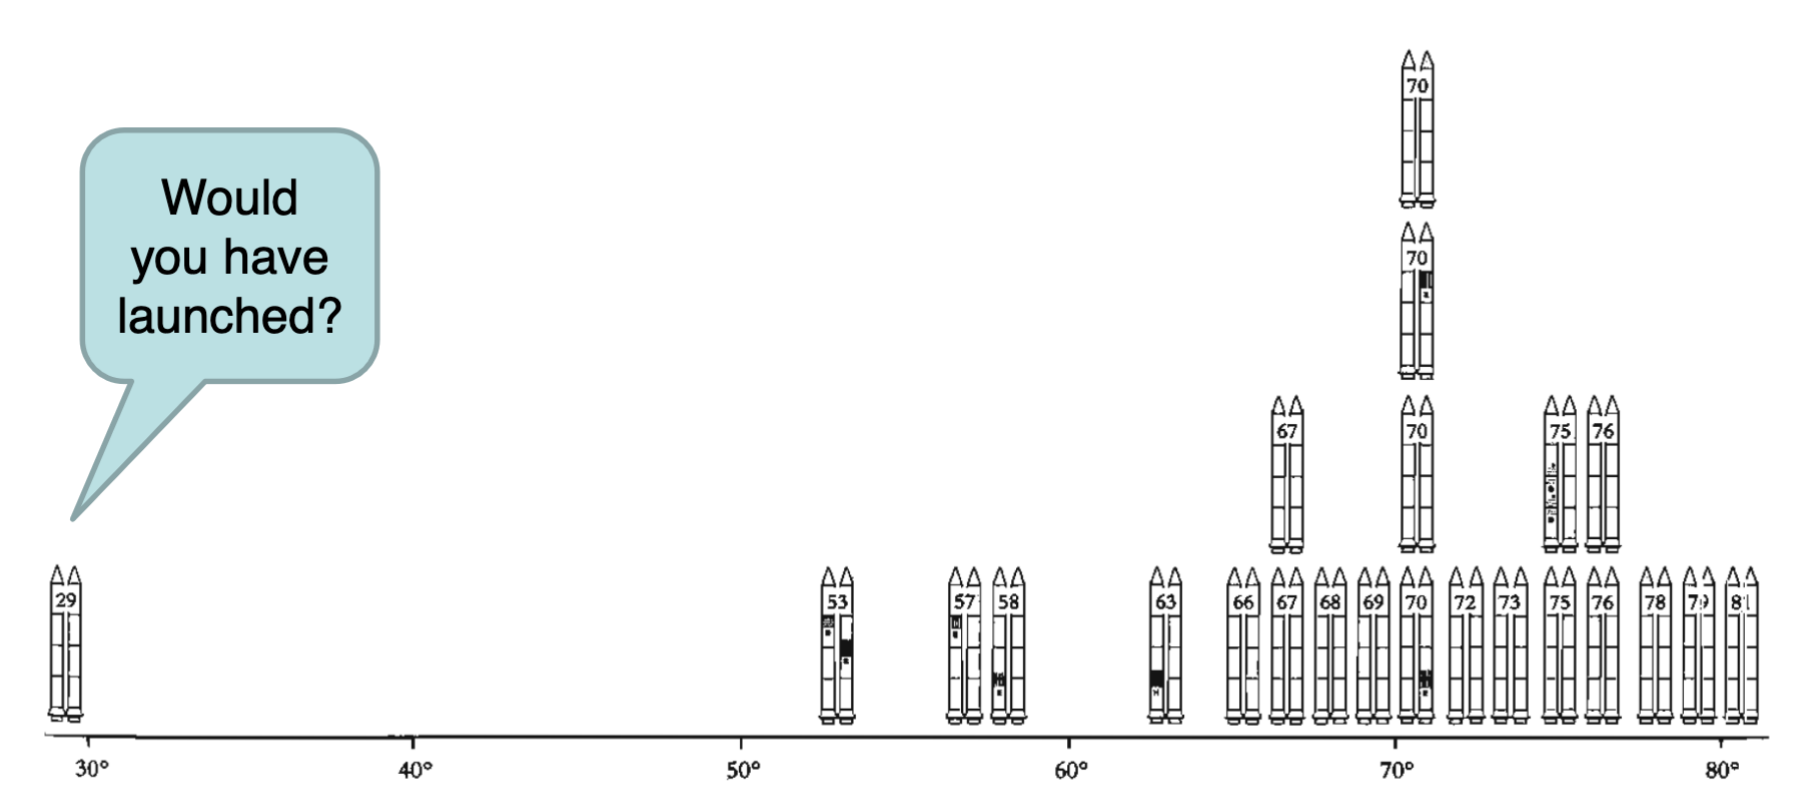
\includegraphics[width=\textwidth]{36.png}

\section{Custom Visualization}

\subsection{Minard’s Map of the 1812 Russian Campaign}
Sometimes you have to construct your own visualization...

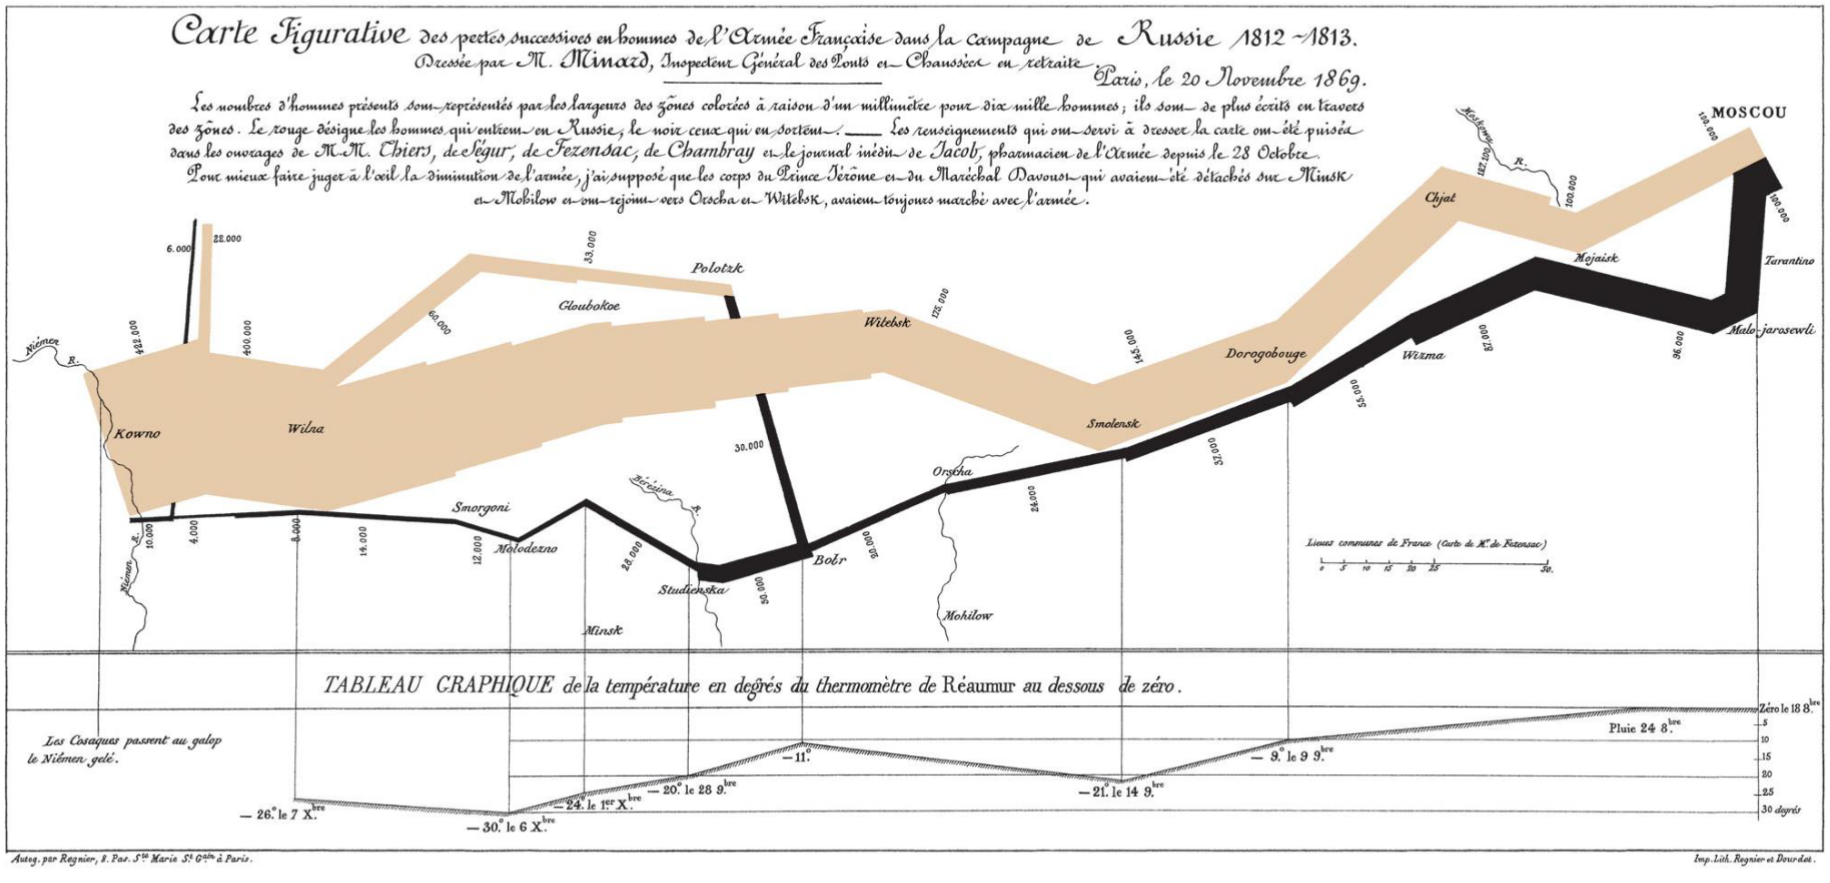
\includegraphics[width=\textwidth]{37.png}

Modern redrawing of Charles Minard's map of Napoleon's disastrous Russian campaign of
1812. The graphic is notable for its representation in two dimensions of six types of data: the
number of Napoleon's troops; distance; temperature; the latitude and longitude; direction of
travel; and location relative to specific dates

\section{Custom Interactive Visualization}
Hans Rosling's Global Temporal Analysis of Life Expectancy and GDP

You want the area to be proportional to the population of the country to better scale quadratically than radius which is linear. 

\section{Dashboards: Real-time Visualization}

Power BI, Tableau work well for visualization.

\section{Debugging
Data-oriented Code}
For machine learning or complex
data science analysis

\subsection{Synthetic Data for Debugging}
\begin{itemize}
    \item Your code will have bugs!
    \item How to debug data analysis / machine learning?
    \begin{itemize}
        \item Make a synthetic dataset
        \begin{itemize}
            \item E.g., (Features x: Age, Gender; Label y: {Snapchat, Facebook})
            \begin{itemize}
                \item Everyone under 20 uses Snapchat
                \item Everyone 20 and over uses Facebook
                \item Random selection for gender
                \item or use label as a feature
            \end{itemize}
            \item Does your analysis uncover the expected trends?
            \item What happens as you add noise?
            \begin{itemize}
                \item 90\%, 80\%, 70\% of people under 20 use Snapchat?
            \end{itemize}
        \end{itemize}
    \end{itemize}
\end{itemize}

Inability to uncover expected trends indicates a bug in your code
or the need to revisit your analysis approach or hypothesis space.

\end{document}